%!TEX root = ../thesis.tex

\chapter{Introduction}
\label{chap:intro}

%Ideas->Describing general picture of melodic analysis for description and characterization of IAM. The one we have used in several presentations.
%Ideas-> When you talk about MIR first say what kinds of varied tasks. And then similarity at diff level and pattern recognition has been a focus since a long time! Talk about glass ceiling in similarities, (ref to Joan's thesis). This maybe because similarities has many variablesm and cultural influence is quite recognized one in that. 
%Ideas-> Our ideas behinf using characteristic phrase is like cover song similarity. There is no comparison between two items for similarity. Its from ones mental abstractino or image. See joan's work to get more insights on how has he presented it.
%Ideas-> read some more thesis on this topic and read intros from PR IITB, they are really good points 
%
%
%Overall what all things
%1) What are in generals the problems that world is facing related with digital music
%2) What if machines can understand music like humans do, what can they do
%
%3) MIR dedicated to this kind of research
%4) Varikous topics, variety of problems, basic research, applied reearch, interdesciplinary, mixture of approaches borrowed from other domains, 
%
%
%Joan's approach: Straight starting from task at hand, motivating need for it --> MIR-->

%
%Basically I want to say that data and information is increasing at a fast pace. We ICT tech that can understand, interpret and make sense of digital data like humans do, so that they can make our interaction with the data and information better. So that we can utilize the data and information better in our lives. Many factors play role here, one of them is the cultural and social context. So bsically those factors should also be taken into account. Once these systems learn how to make sense of data, not only will we be able to consume that better but doing this exercise of making machines make sense of the data can also increase our understanding of the concepts surrounding us. This can also enable novel ways od doing stuff, far suprior than what human do for now. 
%
%

%Technologies that can process digital data to understand and interpret it like humans do have becomes nearly a necessity in modern world. Such technology can not only perform tasks that humans already do but can also pave way for novel ways to interact with the data. During the process of developing such technologies we learn and undertand more about the phenomenon in the world. 


\TODO{Enhance and make it more coherent, also provide a proper endingto connect to the next section}
\Gls{it} is constantly shaping the world that we live in. The advancements in \gls{it} has changed the patterns of human behavior and influenced the way we relate with our environment. The ease with which digital content is generated and shared, further propels the growth of these technologies. Music being a universal socio-cultural phenomena has been deeply influenced by these advancements. In order to respond to the growing need to organize, retrieve and recommend relevant music content, the field of \gls{mir} has advanced rapidly in the last few decades. Music is embedded in a rich web of cultural, historical, commercial and social context, which calls for technologies that take all these perspectives into account. However, a significant part of the technological development in \gls{mir} is based on the western understanding of music, and primarily caters to western commercial music~\citep{XavierSerra2011}. The world is replete with rich music cultures and there is a need to develop culture-aware technologies that help preserve this diversity. Such technologies will not only enable better understanding, accessibility and listening experience of these music cultures but also help push the boundaries of \gls{mir}, expanding its scope and gaining better insights into music in general.



\section{Motivation, Context and Relevance}
\label{sec:intro_motivation_context_relevance}

%Repeating structures are important information units in data such as text, DNA sequences, images, videos, speech and music~\citep{Buhler2002b,Herley2006}. Patterns are exploited in a variety of ways, ranging from signal level tasks such as data-compression~\citep{Atallah1999} to more cognitively complex tasks such as analyzing an art work~\citep{van2010texton}. In music domain, identification of repeating structures in a musical piece is fundamental to its analysis, understanding and interpretation~\citep{Cook1987,Lerdahl1983}. 

\subsection{\titlecap{\glsentrylong{mir}}}
\label{sec:intro_motivation_mir}

\Gls{mir} is a growing interdisciplinary research field that stands at the intersection of well established disciplines such as signal processing, pattern recognition, musicology, psychoacoustics, music perception and cognition, information science, and computer science (machine-learning). \Gls{mir} primarily addresses topics involved in the understanding and modeling of music using information processing methodologies~\citep{roadmap_mir}. In particular, it aims to advance our knowledge in representing, understanding, describing, retrieving, archiving and organizing music related data. This opens up a wealth of possibilities to develop novel ways to interact with music~\citep{casey2008content,orio2006music,burgoyne2016music}. 

%\TODO{remark that we are mainly talking about content based MIR}

The field of \gls{mir} has made significant advancements in the last two decades. However, many of the technologies developed within \gls{mir} are not directly applicable to several music cultures of the world. This can be largely attributed to the fact that the research in \gls{mir} has been mainly focused on the western commercial music of the past few decades~\citep{XavierSerra2011}, which has largely shaped the research problems undertaken in \gls{mir}. A significant effort in \gls{mir} is dedicated towards automatic description and characterization of music content to extract musically and semantically relevant information. Computational approaches in \gls{mir} address a variety of tasks such as melody extraction~\citep{salamon:phd:13}, chord estimation~\citep{mcvicar2014automatic}, music key estimation~\citep{peeters2006chroma}, motif discovery~\citep{collins2011improved,Conklin2010}, music structure analysis~\citep{paulus2010state,serra2012unsupervised}, music similarity~\citep{joan_thesis}, genre classification~\cite{aucouturier2003representing} and emotion recognition~\citep{kim2010music}, tempo and beat tracking~\citep{gouyon2005review,scheirer1998tempo}. These approaches describe and characterize music pieces in terms of different musical aspects such as melody, rhythm, harmony, structure and emotion. The definition, interpretation and relevance of these musical aspects are not universal and vary significantly across different music traditions,  and personal, cultural and social contexts. However, a significant number of existing computational approaches in \gls{mir} fail to account for these factors, and thus, might be hitting the so-called ``glass ceiling"~\citep{pachet2004improving,casey2008content}. This phenomenon is evident from the slowing rate of improvement in the approaches in \gls{mir} over years, as seen in the results of MIREX\footnote{http://www.music-ir.org/mirex/wiki/MIREX\_HOME} evaluations. There also exists a semantic-gap between the automatically extracted music descriptors from audio signals and the high level music concepts that humans relate to~\citep{celma2006foafing,casey2008content}. There is a need to bridge this gap and take a broader perspective to describe music by taking the cultural, social and user context into account~\citep{roadmap_mir}. It is in this context that the CompMusic project was envisioned~\citep{XavierSerra2011}.

%\TODO{highlight lack of knowledge infusion from top dwn. Most approaches work on audio based on features and try to describe higher level concepts}.
\TODO{Should we add some bob sturm stuff? basically to make a point that we try to make human interpretable methods and hence are quite sure that we are not creating horses?}
%
%In addition to the possibility of approaches in \gls{mir} hitting the ``glass ceiling'', there are also growing concerns whether machines are really learning the underlying musical concepts, or are just producing good evaluation results by exploiting features that are musically irrelevant \TODO{ref: bob sturm horse paper}. This becomes evident when a computational method produces drastically different results when fed with different inputs, even when the differences between these inputs are perceptually and musically insignificant\TODO{Genre + deep net ref}.  
%
%Whether intelligent machines should learn to perform a computational task similar to how humans do or not is a topic for a different debate. Irrespective of this, the approaches in \gls{mir} should at least scale to the repertoire on which they are developed and should be invariant to perceptually insignificant low-level transformations.
%
%
%A counter argument to this criticism is to feed a computational method with different transformed variants of the input during the training phase, so that they can be learned and well handled by the system. This is probably true to an extent, but in \gls{mir} it is virtually impossible to work with the whole real-world collection of music and most of the test datasets tend to be a small fraction of that. Therefore, robustness to trivial changes might be important to scale the approaches and systems developed in \gls{mir}. Moreover, one of the motivations of several researchers behind developing such systems is to learn more and get novel insights into music and validate our understanding of music, which might be futile if the systems are not really learning the underlying musical concepts.
%
%
%
%
%\TODO{This paragraph below will be written at some other point where we summarize how we have taken care of these peripheral issues!!}
%In this dissertation we try to steer away from such pitfalls by laying emphasis on the human interpretability of the research results, and wherever possible, of the output of the intermediate stages of our approaches. We are very aware that human interpretability doesn't guarantee that the approaches are generalizable or scalable, but, at least we are conscious of what our systems are learning, which eventually helps to improve them further. In addition, we work with a diverse, representative and sizable collection of \gls{iam} that contains editorial metadata and other relevant information in addition to the audio recordings, which can be regarded as a representative subset of the real-world audio collection of \gls{iam}~(\chapref{chap:corpus_music_corpora_and_datasets}).


%
%\begin{itemize}
%	\item What is music information retrieval
%	\item What is the context in which music information retrieval is growing
%	\item Why is MIR getting more important and finding many applications
%	\item Successful examples of MIR
%	\item What are the different contexts related with music that MIR can help in
%	\item what more?
%\end{itemize}

\subsection{CompMusic Project}
\label{sec:intro_motivation_compmusic}



%To gain insights on the factors responsible for capping the performance of the current \gls{mir} approaches (\secref{sec:intro_motivation_mir}) and to make the research outcome applicable to different music traditions of the world, development of these approaches in a multicultural context is important. 
%
%Note that by this we do not imply that research  in \gls{mir} is only focused on western popular music. There has been work done on analysis of flamenco, folk, ethnomusicology, western classical \TODO{rephrase last line and put references}.

CompMusic\footnote{http://compmusic.upf.edu/} (Computational Models for the Discovery of the World'd Music) is a research project funded by the European Research Council~\citep{XavierSerra2011}. The project focuses on five music traditions of the world: Hindustani (North India), Carnatic (South India), Turkish-makam (Turkey), Arab-Andalusian (Maghreb), and Beijing Opera (China). One of the main objectives of the CompMusic project is to promote and develop multicultural perspectives in \gls{mir}. In particular, the project aims to advance the research in computational description of music by identifying musically relevant problems coming from culture-specific contexts and developing domain specific approaches to solve them. Addressing the research problems in the context of diverse music cultures will not only help in advancing the knowledge in the specific cultures, but also expand the scope of current research in \gls{mir}. Furthermore, it can help bridge the semantic-gap and push the glass-ceiling. 

CompMusic project follows a data-driven research methodology. The efficacy of the computational approaches are directly impacted by the quality of the data using which they are developed. Thus, one of the goals in the CompMusic project is to create good quality data corpora that are representative of real-world music collections. The corpora created in the CompMusic project mainly comprises commercial quality audio recordings and relevant editorial metadata. 

The work presented in this dissertation is carried out as a part of the CompMusic project and aligns with its goals. In this dissertation we focus on computational description and characterization of melodies in \gls{iam}. The cultural specificities of \gls{iam} have shaped our work at every step, whether it is the identification of relevant research problems, building the data corpus, or the methodology adopted for the computational analysis. The insights gained in the process of developing culture-aware approaches for melodic analysis of \gls{iam} will help expand the scope of the research in this domain. Our work paves way for cross-cultural studies, which can help us better understand the influence of cultural training on perception and cognition of different musical aspects. 


%\begin{itemize}
%	\item MIR is important and things are going fine, what's the issue then? Is there any bias in the kind of music tradition being analyzed in MIR right now? whats the reason for this bias
%	\item What kind of music traditions are kind of ignored for anlaysis now?
%	\item What's the reason why no one wants to consider them?
%	\item Is it even relevant to consider them? Which ones amongst them are the easiest ones or the most relevant ones to consider
%	\item Does everyone get benefitted from this kind of work? how things improve overall by doing this?
%	\item What is the objective of COmpMusic project, which music traditions it focuses on. 
%	\item What kind of methodologies are being worked upon in compmusic, What is the main philosophy
%	\item The idea of open-acess and reproducibility
%	\item what more?
%\end{itemize}

\subsection{Computational Melodic Analysis in Indian Art Music}
\label{sec:intro_melodic_analysis_IAM}


\blockcquote{ringer2001melody}{``\textit{Melody, defined as pitched sounds arranged in musical time in accordance with given cultural conventions and constraints, represents a universal human phenomenon traceable to prehistoric times...wherever music became an intrinsic condition of life, certain common melodic procedures were necessarily adopted, because they satisfied basic physiological and biological requirements, if not the aesthetic imagination, per se....`Melodic unity' is configurationally speaking an intrinsic psychoacoustical function of melodic generation in a given historical-cultural context and music in the end be experienced as such...Above all, as a social product, melody is part and parcel of the cultural or subculture to which it owes its existence...}''}

There are two main points to note here; first, that melody is innate to humans and is one of the fundamental aspects in most music traditions, and second, the perception of melody is shaped by cultural influences. Melody is manifested in a number of phenomena that surround us, for example, in lullabies, nursery rhymes, intonation in languages, and music. Melody also facilitates memorization. Historically, when the printed medium was not prevalent, knowledge was transmitted orally across generations, often set to music to make memorization easier. Even today, as listeners, very often we try to reproduce the melody of the song we want to recall. The importance of melody in our musical experiences makes its analysis an interesting topic of research. With no surprises, a significant part of the efforts in music content processing in \gls{mir} is dedicated to the computational analysis of the melodic aspects of music. Such an analysis is even more important for melody dominant music cultures such as \gls{iam} and Flamenco.

The arrangement of the pitched sounds in a melody is shown to be hierarchical in nature\TODO{ref: generative theory}, where the pitched sounds group together into melodic phrases or motifs, which in turn group into sections that together form stanzas finally leading to the musical piece. At each level there is a complex interplay between these different elements of melody. Computational analysis of these melodic elements can provide insights into the musical concepts operating at different levels of abstraction and complexity, and eventually help us automatically extract higher level semantic descriptors \TODO{expand on descriptors and probably some other applications and contexts in which it becomes useful?}.

\textquote*[Cambouropoulos2006]{\textit{Music becomes intelligible to a great extent through self-reference, i.e.,~through the relations of new musical passages to previously heard material. Structural repetition and similarity are crucial devices in establishing such relations}}. Repeating structures or patterns in melodies play a pivotal role in organizing an incoming music stream. \textquote[schenker1980harmony]{Only by repetition can a series of tones be characterized as something definite. Only repetition can demarcate a series of tones and its purpose. Repetition thus is the basis of music as an art}. This makes the computational analysis of melodic patterns and motifs a crucial task in the automatic description of melodies, which is also evident from a large number of studies dedicated to this topic. Discovery of repeated melodic patterns within a music piece (often referred to as intra-opus discovery) can help reveal the structure of the piece, and form the basis for studying the stylistic characteristics of an artist. Such repeating patterns when analyzed at a corpus level can not only help establish similarities between different artists and compositions, but also, facilitate studying stylistic influences across them. 

\TODO{Add the significance of melodic patterns for indian art music, of course we have highlighted it for music in general, but specially for indian art music since its not at the level of a composition but raga its more deep in the sense that it becomes a part of the music theory and its characteristics.}

It is worth noting that the idea of repetition as mentioned above refers to a musical repetition, wherein across occurrences the musical unit can undergo a series of transformations. Few examples of such transformations in the case of melodic patterns are pitch transposition, non-linear time-scaling and addition/deletion of melodic ornaments. A computational approach for pattern discovery should be robust to such transformations. Thus, the task of discovering patterns encapsulates the task of computing similarity in music, which is crucial in developing novel methodologies for music recommendation, navigation and music discovery. As mentioned above, the perception of melody is shaped by the cultural influences. The meaning, interpretation, functional role, relevance and manifestation of the elements of melody as discussed above may significantly differ across music cultures. \TODO{For example, in XXx tradition music is primarily precomposed and hence patterns are a part of the composition and remain more or less the same across occurrences. Whereas, in IAM they are the base for improvisation and are a characteristic of the melodic framework.} For a holistic understanding of these musical concepts it is important that they are studied within a multicultural context.

\TODO{here explain the importance of pattern processing in IAM and of raga recognition. This will be in general irrespective of their peculiarity, problems and challenges...music wise relevance.} 

All the reasons mentioned above \TODO{should we specify the reasons?} motivate us to study computational approaches for the description and characterization of melodies in \gls{iam}. Unavailability or rather inappropriateness of symbolic type music representation, long duration of music performances (sometimes over an hour), distinct melodic characteristics, improvisatory nature of music, and complex melodic framework of \gls{raga} (Section XX) are few peculiar characteristics of \gls{iam} that provide unique opportunities and challenges to expose the shortcomings of the current \gls{mir} systems. Devising novel approaches that overcome these challenges will not only result in making \gls{mir} more accessible to \gls{iam}, but it will also push the boundaries of \gls{mir} technologies. Such computational approaches can enable \gls{raga}-based music retrieval from large audio collections, semantically meaningful music discovery, musically informed navigation and several applications around music pedagogy. In the next section we provide a detailed overview of the challenges and opportunities offered by \gls{iam} in computational analysis of its melodies, which further adds to our motivation behind selecting \gls{iam} for this study.







%
%concept of similaries, and then recommendation and navigation etc
%
%What can we do in practical applications with this this
%
%In the past done this this, since these differ we need to do for indian...
%
%
%These elements, their role, significance and manifestation changes across music cultures. also context changes, many things are diff signal etc...copmlexity is didd. concept of music generation is diff.. improvisation idea is diff...idea of composition is diff
%
%
%
%While a precise objective definition of melody is argued to be impossible (XXX), at a 
%
%Automatic description and characterization of melodies are broad topics with a wide scope that can include a number of computational tasks addressing different aspects of melodies. 
%
%
%Melodies can also be seen as being structured hierarchically according to the melodic framework prevalent in a music tradition. Starting from the basic unit, which is a pitched sound, a note, through a temporal interplay of such events building the whole melody. TYpically arrangement is such that notes group together into phrases, which is a unit that can be considered as a unit incorporating artists thoughts. Silence plays an important role in this structrures and a delimiter. Patterns play an important role in comprehension of melodies and are very important to be studied. It is also linked to lyrics and the strucrture in the lyrics, different lines, stanjas and probably like verses, chorus, which is another hrirarchy of this structure. And then when seen as a whole the fullpiece is basically a piece of art conveying what artist wanted to express and musically is making a unit of a framework (like raga tala). Issue of similarity
%
%Description and characterization are umbrella terms involving a number of computational tasks that act at different levels of abstraction and musical concepts.  Study and analysis of each of these units and different strucrtures at different level is contributing towards description and characterization of melodies. Studing XX is helpgul in XXX and form the basis or input for other tasks. Studying XXX is helpful in blah blah.
%
%
%
%Several different ways to approach description and characterization of music. one of whch is through doing the same for the melody. very widely addressed..
%Automatic analysis for description and characterization of melodies is an imp task, core in mir. examples of the tasks that do that...
%
%Melodies is composed of xxxx, heirarchical arrangement. Tonal and Temporal arramgement. 
%
%One of the ways is pattenr, very imp. 
%
%We can describe at diff level, notes it uses, key and mode, stylistic description, structural description, description of the characterisics
%
%In this thesis focus on patterns. 
%
%what is raga and makam commonly called asd doing that is imp. and why
%
%
%so basically melody is imp, melodic desc is imp, it can help in XXXXXX, it can be at various levels, low level to high level, each one has its own imp, we focus more on patterns, patterns are imp, and why so..then melodic framework, the most abstracted higher level view, we do that too, and since that is closely linked with mood and emotions that directly becomes relevant for recommendation and navigation and those kind of stuff
%
%First time pattern discovery is addressed to this level

description 
\section{Melodic Analysis in Indian Art Music: Challenges and Opportunities}
\label{sec:intro_challenges_oppurtunities}

\TODO{Computational melodic analysis can enable or is advantageous to.....Remove this thesis wala sentence? Rewrite this whole paragraph and give a nice intro to this section.}
The current thesis focuses on developing computational approaches for description and characterization of melodies in \gls{iam}. There are many reasons why such an analysis is relevant for \gls{iam}, and why working on \gls{iam} can help broaden the scope of the current approaches for melody processing in \gls{mir}. In this section we present the main challenges in the computational melodic analysis of \gls{iam}, and the new opportunities that it offers. 


\TODO{Rephrase this paragraph} One of the challenges in computational analysis of \gls{iam} arises from the fact that symbolic music scores corresponding to music performances are practically non existent, and audio recordings are the main data source for computational analysis.  Though, there exists a small repertoire of prescriptive symbolic scores corresponding to musical compositions, the scope and relevance of such music representation in \gls{iam} is practically restricted to its role as a tool for documentation and music training. This is understandable as musical compositions merely act as skeletons in music performances in \gls{iam}, and the essence of the music lies in the improvisatory aspects. In addition, the existing symbolic music representations do not capture the nuances of the melodic material used in the performances of \gls{iam}. \gls{iam} has been transmitted orally across generations and has predominantly followed a tradition of Guru-Shishya parampara (``lineage'' system).  Due to these factors \gls{iam} mainly possesses audio music collections. It is well known in \gls{mir} that computational analysis using audio recordings is challenging and the extraction of a reliable melodic representation from audio signals is still an active topic of research. However, working with the audio music collections of \gls{iam} can be seen as an opportunity.  The extraction of predominant melody in audio recordings of \gls{iam} appears to be relatively easier compared to the other music traditions such as rock, jazz and orchestral music. This performance difference is evident from the MIREX results\footnote{\TODO{link?}}. It can be attributed to the fact that a performance of \gls{iam} typically involves a small number of simultaneously playing musical instruments compared to other music traditions, resulting into a sparse polyphonic audio content, which is easier to process for the melody extraction algorithms. In addition, since \gls{iam} is a melody dominant tradition and comprises largely vocal-based music, the lead voice is predominant compared to the accompanying instruments. These factors make the extraction of predominant melody in \gls{iam} relatively easier. Thus, \gls{iam} provides an opportunity to broaden the scope of current pattern-based melodic analysis approaches, and make advancements in computational melodic analysis in audio music collections.

\begin{figure}
	\begin{center}
		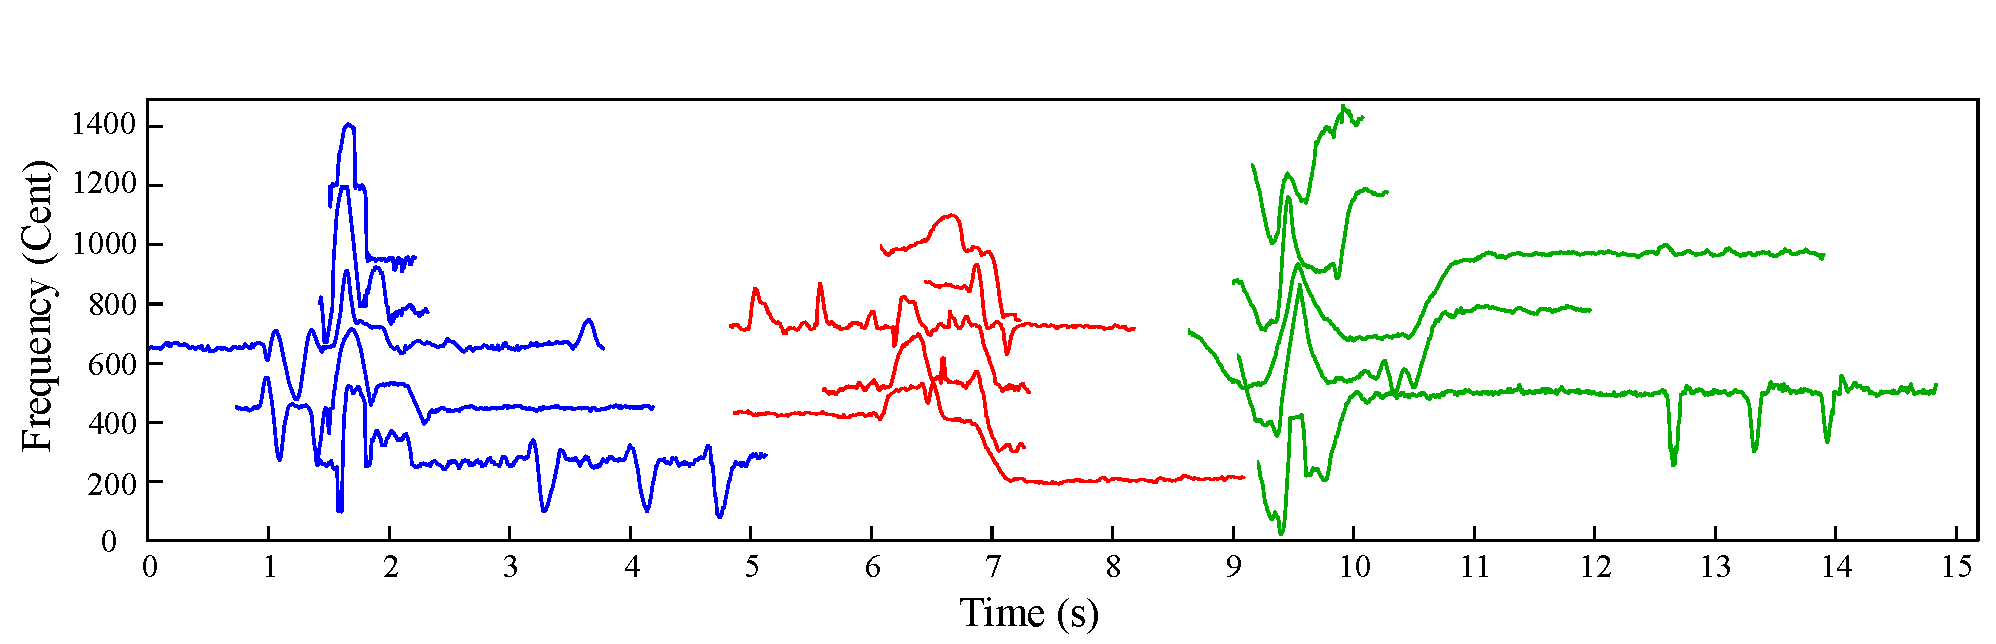
\includegraphics[width=\figSizeHundred]{ch01_introduction/figures/phraseClassesExample.pdf}
	\end{center}
	\caption{Pitch contours of occurrences of three different characteristic melodic phrases in Hindustani music. Contours are frequency transposed and time shifted for a better visualization.\TODO{diff aspect ratio?}}
	\label{fig:phraseComplexityExample_intro}
\end{figure}

An aspect that makes processing of melodies in \gls{iam} both interesting and challenging at the same time is the improvisatory nature of the music. The characteristic melodic phrases of \glspl{raga} (Section XX) act as the basis for artists to improvise, providing them with a medium to express creativity during \gls{raga} rendition. Since the essence of this music lies largely in the improvisatory aspects, artists bring in novelty through creatively transforming these melodic phrases as much as possible within the periphery defined by the \gls{raga} grammar. Therefore, the surface representation of these melodic phrases vary a lot across their occurrences. This high degree of variation in terms of the overall duration of a phrase, non-linear time warpings and the added melodic ornaments together pose a big challenge for melodic similarity computation and pattern extraction in \gls{iam}. In~\figref{phraseComplexityExample_intro} we illustrate this variability by showing the pitch contours of the different occurrences of three characteristic melodic phrases of the \gls{raga} Alaiya Bilawal. We can clearly see that the duration of a phrase across its occurrences varies a lot and the steady melodic regions are highly varied in terms of the duration and the presence of melodic ornaments. Thus, due to the improvisatory nature of the music, pattern processing in melodies of \gls{iam} becomes a challenging task. This context provides an opportunity to gain deeper insights into the perception of melodic similarity as well as how it is influenced by different cultural aspects. 

Melodic characteristics in \gls{iam} differ significantly from a lot of other music traditions that are often the focus of studies in \gls{mir}. One peculiar characteristic of  melodies in Carnatic music (Section XX) is the meandering movement of the predominant pitch. Such melodic characteristics pose a challenge to melody transcription, a step often involved in the process of the abstraction of melody. In addition, since these rapid pitch movements are characteristic aspect of melodic patterns they need to be preserved while computing melodic similarity, implying a fine grained representation of melody. Using a fine grained continuous predominant pitch representation of melody makes the task of pattern discovery further more difficult because of the computational complexity involved in the task.

%A beat level summarization of features, which is often performed in a number of tasks in \gls{MIR} to reduce the time-series dimensionality is not suited for melodies in \gls{iam}. 

%As mentioned, a composition mainly acts as a skeleton or a framework for an artist to construct a melody. In fact, typically the opening unmetered section, \gls{alap}, is not not based on any composition but is completely improvised. 

A vast majority of approaches for pattern processing in music focus on intra-opus or intra-recording pattern discovery. Since computational complexity is often one of the primary concerns in such a task, long duration of the performances in \gls{iam} pose a unique challenge. For the long duration audio recordings lasting around an hour computational of self similarity becomes a computationally challenging task. To better understand the magnitude of computational complexity, consider a predominant pitch sequence of an hour long recording, sampled at 50\,Hz\footnote{a near-optimal sampling rate reported in \secref{sec:patterns_evaluation_of_similarity_measures}}. The pitch sequence comprises $1.8x10^{5}$ number of samples, which in turn amounts to nearly $3.2x10^{10}$ cells in the self similarity matrix. \XXX{S}{J}{Is this a strong point? how can we make it impressive} Thus, long performances in \gls{iam} introduce another set of challenges to this task. However, at the same time it is an opportunity as it provides a use-case to devise and test scalable approaches for pattern discovery from audio recordings. 


%Techniques that are typically employed to reduce the computational complexity in pattern processing task are; transcribe the melody to generate a symbolic score like representation and considering dimensionality reduced version of the feature, usually done through beat duration averaging. Applicability of both these techniques is questionable in the context of \gls{iam} owing the melodic characteristics. Melodic transcription is very complex and an ill defined task for melodic in \gls{iam}. And beat level summarization is musically not relevant since we are intersted in considering fine grained melodic nuances in the computation of melodic similarity. Moreover, estimation of beat locations is a  \TODO{complete it nicely}

\TODO{we are looking after really short duration patterns, that is also another challenge, please note that. Also typically beat summarization is done to reduce computational complexity, that can't be done here because 1) we wnt to present melodic nuances as the yare imp for simlarity and beat restimation is hard. Also for very small duration pattern that doesn't make sense....}


There is no standard frequency that is used as a reference for tuning instruments and voice in a music performances of \gls{iam}. The tonic pitch of the lead artist acts as the base frequency using which all the other instruments are tuned. Tonic pitch varies across artists and may vary across the different performance of an artist. In addition, an artist is free to choose any arbitrary frequency as a tonic in a performance. This aspect of music performance in \gls{iam} makes it difficult to directly compare melodies across different artists and audio recordings. 

There are many music traditions in the world where the manifestations of the seemingly transversal musical concepts such as melody and rhythm present a wide range of challenges to the current computational approaches in \gls{mir}. However, a very important factor behind selecting \gls{iam} for this analysis is the existence of musicological literature and well established music theory. \gls{iam} is an old music tradition whose origins can be traced back to the Vedas dating back to 1500 BCE. With that history, musical concepts in \gls{iam} are well studied and there exists a rich literature. This can be regarded as an opportunity, since basing the methodologies on the established music theories can speed up the advancements of computational approaches. 



%However at the same time not every computational task can directly benefit from the existing music theory. For example, the theory behind the concept of \gls{raga} in \gls{iam} elaborates WTF is happening to my mind!!!!!

%In this dissertation our focus is from an engineering perspective and solely on the computational aspects, we take established music theories for granted. Notably that is one major difference between an analysis like ours and studies in ethno-musicollogical. 


These challenges and opportunities offered by \gls{iam} sets in a unique context to develop novel methodologies for computational melodic anlaysis, and thus, improve the current state of the art in \gls{mir}. 






%
%\begin{itemize}
%	\item in general music similaity, search and discovery. Different applications and context
%	\item melodic analysis->representation of tonal content often used->melodic representaiton->difficulaty in extraction
%	\item problems which are solved by the state of the art in melody extraction for different music types
%	\item for which music types melodic anlaysis make more sense and have been done successfully.
%	\item Symbolic domain research, a lot of work.
%	\item Key detection and cover song detection.
%\end{itemize}
%
%\begin{itemize}
%	\item Music similarity focus in MIR
%	\item application and context of music similarity
%	\item how that has given rise to search and discovery in different contexts
%	\item use cases/ applications / relevant problems within similarity and search and discovery
%\end{itemize}

\section{Scope and Objectives}
\label{sec:intro_scope_context_relevance}

In this section we define the scope of our research work, clearly outline our objectives and enumerate the research questions addressed in this dissertation. 

Computational description and characterization of melodies is a broad research topic that can be approached from a number of perspectives involving different disciplines of science. In this dissertation we take a data-driven engineering approach and focus solely on the computational aspects of melodic analysis, building on top of established music theories. Our applied research methodology, stands at an intersection of signal processing, machine learning and time-series analysis. We focus on content-based processing and the input data used in our approaches comprise audio recordings. The only exception to this is the approach described in~\secref{sec:patterns_characterization_of_melodic_patterns}, which utilize the associated editorial metadata of the recordings in addition to the audio data. The approaches proposed in this thesis are devised and evaluated on music collections in \gls{iam} that includes both Hindustani and Carnatic music. We now outline our broad objectives in this dissertation.

\begin{itemize}
	\item To build a representative music corpora of \gls{iam} that comprises audio recordings and relevant editorial metadata, and use that to compile sizable and well annotated tests datasets for melodic analyses.
	\item To devise a data-driven computational approach to discover musically relevant melodic patterns in sizable audio collections of \gls{iam}
	\item To devise culture-aware and human interpretable approaches for automatic \gls{raga} recognition.
\end{itemize}


\TODO{enumerate all these tasks} There are a number of research tasks within computational melodic analysis that are addressed in this dissertation, which sum up to achieve our broad objectives. We list these tasks in~\figref{fig:tasks}, starting from the bottom and building to the top. We now provide a brief description of these specific tasks to show their relation and relevance in our broad objectives. 

\begin{figure}[h]
	\begin{center}
		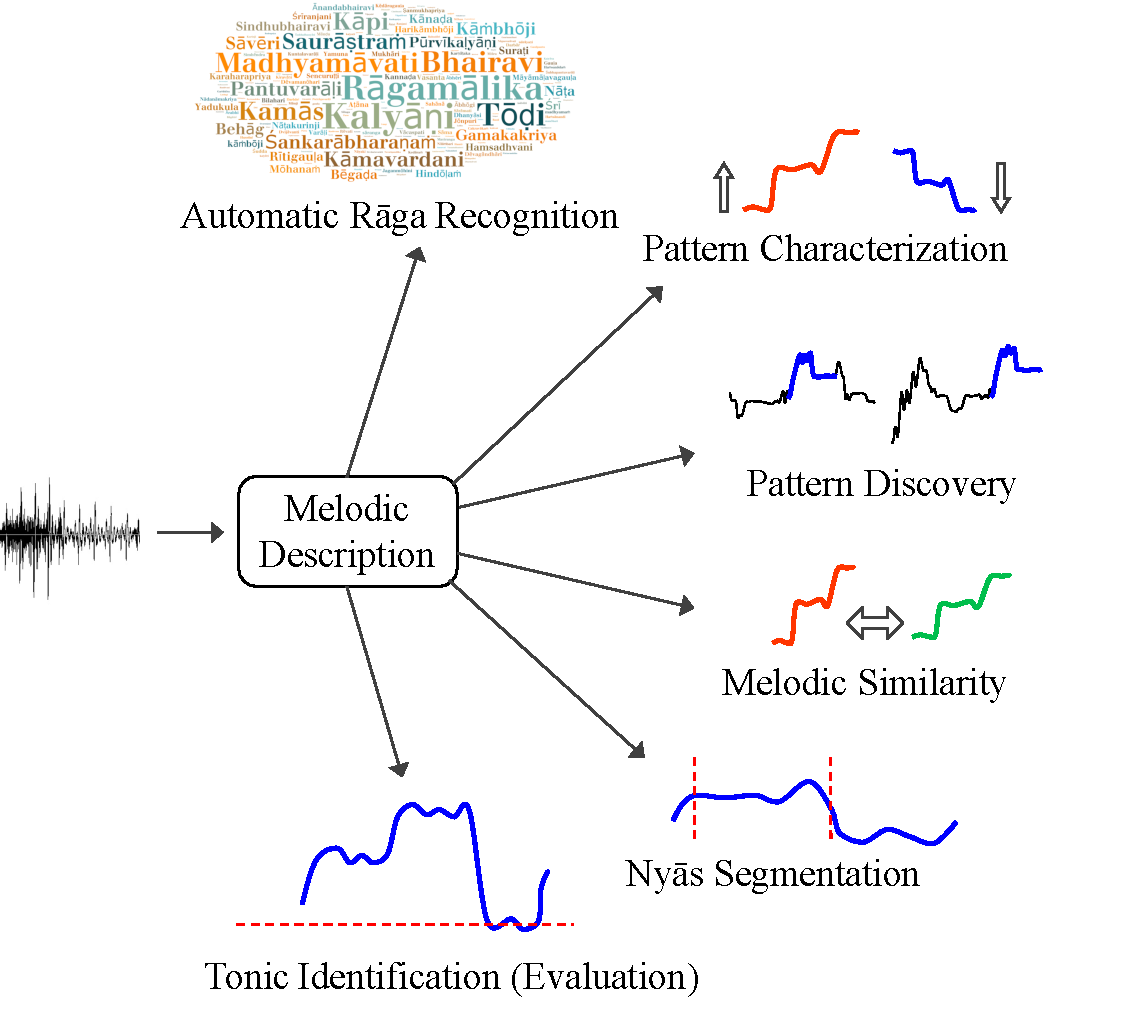
\includegraphics[width=\figSizeHundred]{ch01_introduction/figures/tasks.pdf}
	\end{center}
	\caption{Computational tasks within melodic analysis of \gls{iam} addressed in this dissertation.}
	\label{fig:tasks}
\end{figure}

As mentioned before, tonic pitch of the lead artist in a performance is the base frequency used for tuning by other instruments. For a meaningful comparison of melodies across artists and their recordings, identification of the tonic pitch in a recording is a fundamental task. In recent years a number of methods are proposed for tonic identification, however, there is no consensus on the best performing approach since the evaluations are performed on different datasets, under different experimental conditions. We address this issue by performing an extensive comparative evaluation of seven different tonic identification methods on six diverse datasets of \gls{iam} and identify the approaches that are robust and more accurate on both Hindustani and Carnatic music. In the process we also gain valuable insights into the types of errors made by tonic identification approaches, a useful information while devising methods that require tonic of the recordings as one of the inputs.

Melody segmentation is an important and a well researched topic in melody description in \gls{mir}. It is a crucial step in pattern processing tasks, specifically in the task of discovering melodic patterns. To the best of our knowledge, there are no computational approaches that directly address phrase segmentation in melodies of \gls{iam} from audio recordings\footnote{At the time of starting of this thesis work, 2012}. It is well known from musicological studies that \gls{nyas} \gls{svara} occurrences mark the boundaries of characteristic melodic phrases of \glspl{raga} in melodies of Hindustani music. Thus, detection of such segments in melodies can be an approach to melodic segmentation. We therefore address the task of automatically segmenting \gls{nyas} \gls{svara} segments in the melodies of Hindustani music. 

Musically meaningful computation of melodic similarity is one of the most crucial steps in melodic pattern extraction. Since the task of melodic pattern discovery follows an unsupervised approach, its quantitative evaluation on sizable music collections is a challenging task. As a result of which, evaluation of the methods used for computing melodic similarity also becomes difficult. Computation of melodic similarity in \gls{iam} is a work in progress and it has gained popularity during the course of this thesis. While addressing the task of computing melodic similarity in \gls{iam} we aim to clearly understand the challenges involved in the task, to analyze quantitatively the influence of different processing steps and parameter values on the accuracy, and to finally select the best possible method that can be used for the pattern discovery task. Our main intention behind investigating melodic similarity is to bootstrap our approach for melodic pattern discovery. 

We subsequently address the task of pattern discovery from large audio collections of \gls{iam}, which is one of the main objectives in this dissertation. In melodic pattern discovery we aim to extract all kinds of repeated melodic patterns, which can correspond to different types of melodic units in \gls{iam} with varying degree of musical relevance. In order to successfully use the discovered melodic patterns in analyzing high-level musical concepts such as \gls{raga}, it becomes important to assess the musical relevance of the discovered patterns. We therefore address the task of pattern characterization to identify the musically most relevant melodic patterns, the characteristic phrases of \glspl{raga}.

Finally, we investigate one of the most studied and relevant topics in computational anlaysis of \gls{iam}, automatic \gls{raga} recognition. We aim to devise a culturally-aware approach utilizing the main cues that listeners of \gls{iam} exploit to recognize \glspl{raga}. 

This work in this thesis is done as a part of the CompMusic project, and it aligns with the goals of the project. The objectives of this thesis are directed towards a bigger goal of developing culture-aware computational approaches that can utilize domain knowledge in order to produce semantically meaningful description of music. This thesis is also well aligned with the project's philosophy of open-access and reproducible research. All the data and code used to produce the results reported in this thesis is made openly available, with the exception of the commercial recordings, which is made accessible through personal contact\TODO{Ask xavier what to write!!}. In addition, whenever possible, we also make the output of our methods available to further facilitate reproducing the research results reported in this thesis.


\TODO{Should we be writing specific research questions???? given that our work is quite applied. Ask Xavier and Joan and then decide!!}


\section{Organization and Outline of the thesis}
\label{sec:intro_organization}

There are eight chapters in this thesis. However, the primary contributions are contained in four chapters, Chapter\,3 to Chapter\,6. Each of these four chapters contain one main topic of this thesis, data corpus and datasets, data pre-processing procedures, melodic pattern processing and \gls{raga} recognition. A significant amount of the content in these chapters is derived from our peer-reviewed research papers~\cite{Gulati2014Tonic,gulati2014Landmark,gulati_SITIS_2014,gulati_ICASSP2015,gulati_ISMIR_2015,gulati_communities_2016,gulatiphrase_2016,gulati_tdms_2016}. Most of the work in these papers is done in collaboration with other researchers and musicians, which is duly indicated wherever required. We now proceed to describe a detailed outline of this thesis.

In \chapref{chap:background}, we provide an overview of the music and scientific background and review relevant literature available on the topics addressed in this thesis. We begin with a short description of the terminology used in this thesis. We then provide a brief introduction to \gls{iam} and of the music concepts directly related to melodic aspects in this music tradition. We review existing research within \gls{mir} that relate to the topics covered in this dissertation. We analyze separately the literature that focuses on computational analysis of \gls{iam} and the one for other music traditions of the world. We finally present an overview of the relevant scientific background needed to better understand the technical concepts discussed in this thesis. Our main contribution in this chapter is in reviewing the relevant literature and compiling it.

In \chapref{chap:corpus_music_corpora_and_datasets}, we present an overview of the music corpora and test datasets of \gls{iam} that are compiled as a part of the CompMusic project. We enumerate the set of design criterion followed to build music corpora for research in \gls{iam}~\citep{serra:14:corpus}. We describe both Hindustani and Carnatic music corpus and present a short evaluation of the goodness of the corpora with respect to different criterion. Subsequently, a detailed description of the individual test datasets used for evaluations in this thesis is provided. The content of this chapter is derived from~\citep{serra:14:corpus,CM_Corpora_Ajay14}. Our main contributions in this chapter are in building the research corpora, which was a team effort, and compiling and annotating different test datasets with the help from musicians.

In \chapref{chap:data_preprocessing}, we describe different data pre-processing blocks employed in our work to obtain musically relevant melody representations and descriptors that will be used by the methods described in the subsequent chapters. The main goal in this chapter is to present an extensive comparative evaluation of the available tonic identification approaches to select the best approach that will be used in this work, and to present our novel method for \gls{nyas} segmentation in melodies of \gls{iam}. These two tasks primarily cover our novel contributions in this chapter. In addition, we also present an overview of the methods that we use to obtain a melody representation from audio recordings.

In \chapref{chap:melodic_pattern_processing}, we present our main contributions in melodic pattern processing in \gls{iam}. There are three related topics discussed in this chapter, melodic similarity, pattern discovery and pattern characterization. We first investigate relevant melodic similarity measures with an objective to learn the influence of different choices of melody representation, distance measure and normalization strategy on melodic similarity computation for characteristic melodic patterns of \glspl{raga}. In the process we propose a novel approach to improve melodic similarity by exploiting specific characteristics of melodies in \gls{iam}. Having learned the optimal set of procedures and system parameters in an supervised setup, we utilize this knowledge for discovering melodic patterns in audio collections of \gls{iam}, in which we follow an unsupervised methodology. Finally, we discuss a novel approach to characterize the discovered melodic patterns in order to identify the ones that correspond to \gls{raga} motifs. All four studies reported in this chapter are based on our novel contributions.

In \chapref{chap:raga_recognition}, we present the other significant part of our scientific contributions in the thesis. This chapter addresses one of the most studied topics in computational analyses of \gls{iam}, automatic \gls{raga} recognition. We propose two novel approaches for \gls{raga} recognition. Our first approach utilizes melodic patterns, which are the most prominent cues for \gls{raga} recognition used by the human listeners. We utilize the discovered melodic patterns from previous chapter and employ vector space modeling techniques to model \glspl{raga}. In our second approach we propose a novel melodic representation inspired by the concept of delay coordinates. This representation encodes both the tonal and the temporal aspects of melodies that are relevant to characterize \glspl{raga}. We perform comparative evaluations with the existing methods and show that our system outperforms state of the art by significant margins.

In \chapref{sec:applicatoins}, we present applications and a demo that are based on the research outcomes in CompMusic, which also includes the work done in this thesis. In particular, we introduce Dunya, a web-based research prototype that exposes the resarch outcomes and resources in the CompMusic project and consolidates the tools and technology developed in the project. We provide a brief description of both the interfaces, web-interface and web-API, that Dunya offers to access the content. In addition, we introduce two real-world applications; Saraga and Riyaz, that capitalize on our research outcomes in CompMusic and cater to two types of use-cases, enhance listening and music education. In order to demonstrate the outcome of our melodic pattern processing approaches more directly, we also present a web-based demo. It shows a network-based navigation across discovered melodic patterns and audio recordings. \TODO{written very roughly change it after you have more idea of that chapter}

At the end of every chapter listed above we present a summary of the results and conclusions. Finally, in \chapref{sec:conclusoins} we present the overall conclusions of this thesis work, list our main contributions and discuss possible future directions for improving melodic description of \gls{iam}. This thesis also contains three appendix sections. Appendix A, lists the publications by the author, Appendix B, present ways to access the relevant resources and Appendix C, presents the glossary of the abbreviations and other terms used in this thesis.














